\documentclass{scrreprt}

\usepackage{aligned-overset}
\usepackage{amsmath}
\usepackage{amssymb}
\usepackage{bm}
\usepackage[shortlabels]{enumitem}
\usepackage{hyperref}
\usepackage[utf8]{inputenc}
\usepackage{listings}
\usepackage{multicol}
\usepackage{mathtools}
\usepackage{physics}
\usepackage{stmaryrd}
\usepackage{longtable}
\usepackage{tabularx}
\usepackage{titling}
\usepackage{fancyhdr}
\usepackage{xfrac}
\usepackage{pgfplots}

\pgfplotsset{compat = newest}
\usetikzlibrary{intersections}
\usetikzlibrary{patterns}
\usetikzlibrary{positioning}
\usetikzlibrary{shapes.misc}
\usepgfplotslibrary{fillbetween}

\author{Karsten Lehmann}
\date{WiSe 2021/2022}
\title{Übungsblatt 10\\Algorithmen und Datenstrukturen}

\setlength{\headheight}{26pt}
\pagestyle{fancy}
\fancyhf{}
\lhead{\thetitle}
\rhead{\theauthor}
\lfoot{\thedate}
\rfoot{Seite \thepage}

\begin{document}
\paragraph{Aufgabe 2}
Der gerichtete Graph $G$ sei durch folgende Darstellung gegeben:

\begin{tikzpicture}
  \node[circle, draw] (1) {1};
  \node[below left = of 1, circle, draw] (2) {2};
  \node[below right = of 1, circle, draw] (8) {8};
  \node[below = 0.7 of 1, circle, draw] (10) {10};
  \node[below = of 2, circle, draw] (3) {3};
  \node[below = 0.95 of 10, circle, draw] (9) {9};
  \node[below = of 8, circle, draw] (7) {7};
  \node[below = of 3, circle, draw] (4) {4};
  \node[below = of 9, circle, draw] (5) {5};
  \node[below = of 7, circle, draw] (6) {6};
  \draw[->] (1) -- (2);
  \draw[->] (2) -- (3);
  \draw[->] (3) -- (4);
  \draw[->] (4) -- (5);
  \draw[->] (5) -- (6);
  \draw[->] (6) -- (7);
  \draw[->] (7) -- (8);
  \draw[->] (10) -- (2);
  \draw[->] (10) -- (8);
  \draw[->] (2) -- (9);
  \draw[->] (9) -- (4);
  \draw[->] (1) -- (8);
  \draw[->] (8) -- (9);
  \draw[->] (9) -- (6);
\end{tikzpicture}

\begin{enumerate}[a)]
\item Wenden Sie auf G wiederholt den DFS-Algorithmus mit dem Startknoten 1 an
  und bestimmen Sie auf diese Weise drei unterschiedliche \emph{depth-first-trees}.

  \subparagraph{Lsg.} \:\\
  \begin{longtable}{p{0.2\textwidth}|c}
    Keller & depth-first-tree \endhead
    \hline
    $\qty\big[(1, 2), (1, 8)]$ &
    \begin{tikzpicture}
      \node[circle, draw] {1};
    \end{tikzpicture} \\
    \hline
    $\qty\big[(2, 3), (2, 9), (1, 8)]$ &
    \begin{tikzpicture}
      \node[circle, draw] (1) {1};
      \node[below left = 0.3 of 1, circle, draw] (2) {2};
      \draw[->] (1) -- (2);
    \end{tikzpicture} \\
    \hline
    $\qty\big[(3, 4), (2, 9), (1, 8)]$ &
    \begin{tikzpicture}
      \node[circle, draw] (1) {1};
      \node[below left = 0.3 of 1, circle, draw] (2) {2};
      \node[below = 0.3 of 2, circle, draw] (3) {3};
      \draw[->] (1) -- (2);
      \draw[->] (2) -- (3);
    \end{tikzpicture} \\
    \hline
    $\qty\big[(4, 5), (2, 9), (1, 8)]$ &
    \begin{tikzpicture}
      \node[circle, draw] (1) {1};
      \node[below left = 0.3 of 1, circle, draw] (2) {2};
      \node[below = 0.3 of 2, circle, draw] (3) {3};
      \node[below = 0.3 of 3, circle, draw] (4) {4};
      \draw[->] (1) -- (2);
      \draw[->] (2) -- (3);
      \draw[->] (3) -- (4);
    \end{tikzpicture} \\
    \hline
    $\qty\big[(5, 6), (2, 9), (1, 8)]$ &
    \begin{tikzpicture}
      \node[circle, draw] (1) {1};
      \node[below left = 0.3 of 1, circle, draw] (2) {2};
      \node[below = 0.3 of 2, circle, draw] (3) {3};
      \node[below = 0.3 of 3, circle, draw] (4) {4};
      \node[right = 0.1 of 4, circle, draw] (5) {5};
      \draw[->] (1) -- (2);
      \draw[->] (2) -- (3);
      \draw[->] (3) -- (4);
      \draw[->] (4) -- (5);
    \end{tikzpicture} \\
    \hline
    $\qty\big[(6, 7), (2, 9), (1, 8)]$ &
    \begin{tikzpicture}
      \node[circle, draw] (1) {1};
      \node[below left = 0.3 of 1, circle, draw] (2) {2};
      \node[below = 0.3 of 2, circle, draw] (3) {3};
      \node[below = 0.3 of 3, circle, draw] (4) {4};
      \node[right = 0.1 of 4, circle, draw] (5) {5};
      \node[right = 0.1 of 5, circle, draw] (6) {6};
      \draw[->] (1) -- (2);
      \draw[->] (2) -- (3);
      \draw[->] (3) -- (4);
      \draw[->] (4) -- (5);
      \draw[->] (5) -- (6);
    \end{tikzpicture} \\
    \hline
    $\qty\big[(7, 8), (2, 9), (1, 8)]$ &
    \begin{tikzpicture}
      \node[circle, draw] (1) {1};
      \node[below left = 0.3 of 1, circle, draw] (2) {2};
      \node[below = 0.3 of 2, circle, draw] (3) {3};
      \node[below = 0.3 of 3, circle, draw] (4) {4};
      \node[right = 0.1 of 4, circle, draw] (5) {5};
      \node[right = 0.1 of 5, circle, draw] (6) {6};
      \node[above = 0.3 of 6, circle, draw] (7) {7};
      \draw[->] (1) -- (2);
      \draw[->] (2) -- (3);
      \draw[->] (3) -- (4);
      \draw[->] (4) -- (5);
      \draw[->] (5) -- (6);
      \draw[->] (6) -- (7);
    \end{tikzpicture} \\
    \hline
    $\qty\big[(8, 9), (2, 9), (1, 8)]$ &
    \begin{tikzpicture}
      \node[circle, draw] (1) {1};
      \node[below left = 0.3 of 1, circle, draw] (2) {2};
      \node[below = 0.3 of 2, circle, draw] (3) {3};
      \node[below = 0.3 of 3, circle, draw] (4) {4};
      \node[right = 0.1 of 4, circle, draw] (5) {5};
      \node[right = 0.1 of 5, circle, draw] (6) {6};
      \node[above = 0.3 of 6, circle, draw] (7) {7};
      \node[above = 0.3 of 7, circle, draw] (8) {8};
      \draw[->] (1) -- (2);
      \draw[->] (2) -- (3);
      \draw[->] (3) -- (4);
      \draw[->] (4) -- (5);
      \draw[->] (5) -- (6);
      \draw[->] (6) -- (7);
      \draw[->] (7) -- (8);
    \end{tikzpicture} \\
    \hline
    $\qty\big[(2, 9), (1, 8)]$ &
    \begin{tikzpicture}
      \node[circle, draw] (1) {1};
      \node[below left = 0.3 of 1, circle, draw] (2) {2};
      \node[below = 0.3 of 2, circle, draw] (3) {3};
      \node[below = 0.3 of 3, circle, draw] (4) {4};
      \node[right = 0.1 of 4, circle, draw] (5) {5};
      \node[right = 0.1 of 5, circle, draw] (6) {6};
      \node[above = 0.3 of 6, circle, draw] (7) {7};
      \node[above = 0.3 of 7, circle, draw] (8) {8};
      \node[below left = 0.5 and 0.3 of 8, circle, draw] (9) {9};
      \draw[->] (1) -- (2);
      \draw[->] (2) -- (3);
      \draw[->] (3) -- (4);
      \draw[->] (4) -- (5);
      \draw[->] (5) -- (6);
      \draw[->] (6) -- (7);
      \draw[->] (7) -- (8);
      \draw[->] (8) -- (9);
    \end{tikzpicture} \\
    \hline
    $\qty\big[]$ &
    \begin{tikzpicture}
      \node[circle, draw] (1) {1};
      \node[below left = 0.3 of 1, circle, draw] (2) {2};
      \node[below = 0.3 of 2, circle, draw] (3) {3};
      \node[below = 0.3 of 3, circle, draw] (4) {4};
      \node[right = 0.1 of 4, circle, draw] (5) {5};
      \node[right = 0.1 of 5, circle, draw] (6) {6};
      \node[above = 0.3 of 6, circle, draw] (7) {7};
      \node[above = 0.3 of 7, circle, draw] (8) {8};
      \node[below left = 0.5 and 0.3 of 8, circle, draw] (9) {9};
      \draw[->] (1) -- (2);
      \draw[->] (2) -- (3);
      \draw[->] (3) -- (4);
      \draw[->] (4) -- (5);
      \draw[->] (5) -- (6);
      \draw[->] (6) -- (7);
      \draw[->] (7) -- (8);
      \draw[->] (8) -- (9);
    \end{tikzpicture} \\
    \hline
  \end{longtable}

  Alternativ, wenn man zuerst der rechten Kante folgt:

  \begin{tikzpicture}
    \node[circle, draw] (1) {1};
    \node[below left = 0.3 of 1, circle, draw] (2) {2};
    \node[below = 0.3 of 2, circle, draw] (3) {3};
    \node[below = 0.3 of 3, circle, draw] (4) {4};
    \node[right = 0.1 of 4, circle, draw] (5) {5};
    \node[right = 0.1 of 5, circle, draw] (6) {6};
    \node[above = 0.3 of 6, circle, draw] (7) {7};
    \node[above = 0.3 of 7, circle, draw] (8) {8};
    \node[below left = 0.5 and 0.3 of 8, circle, draw] (9) {9};
    \draw[->] (1) -- (8);
    \draw[->] (8) -- (9);
    \draw[->] (9) -- (6);
    \draw[->] (6) -- (7);
    \draw[->] (1) -- (2);
    \draw[->] (2) -- (3);
    \draw[->] (3) -- (4);
    \draw[->] (4) -- (5);
  \end{tikzpicture}

  Oder wenn man abwechselnd der linken und rechten Kante folgt:

  \begin{tikzpicture}
    \node[circle, draw] (1) {1};
    \node[below left = 0.3 of 1, circle, draw] (2) {2};
    \node[below = 0.3 of 2, circle, draw] (3) {3};
    \node[below = 0.3 of 3, circle, draw] (4) {4};
    \node[right = 0.1 of 4, circle, draw] (5) {5};
    \node[right = 0.1 of 5, circle, draw] (6) {6};
    \node[above = 0.3 of 6, circle, draw] (7) {7};
    \node[above = 0.3 of 7, circle, draw] (8) {8};
    \node[below left = 0.5 and 0.3 of 8, circle, draw] (9) {9};
    \draw[->] (1) -- (2);
    \draw[->] (2) -- (9);
    \draw[->] (9) -- (4);
    \draw[->] (4) -- (5);
    \draw[->] (5) -- (6);
    \draw[->] (6) -- (7);
    \draw[->] (7) -- (8);
    \draw[->] (2) -- (3);
  \end{tikzpicture}

\item Wenden Sie auf G wiederholt den BFS-Algorithmus mit dem Startknoten 1 an
  und bestimmen Sie auf diese Weise drei unterschiedliche
  \emph{breadth-first-trees}.

  \subparagraph{Lsg.} \:\\
  \begin{longtable}{p{0.2\textwidth}|c}
    Keller & depth-first-tree \endhead
    \hline
    $\qty\big[(1, 2), (1, 8)]$ &
    \begin{tikzpicture}
      \node[circle, draw] {1};
    \end{tikzpicture} \\
    \hline
    $\qty\big[(2, 3), (2, 9), (8, 9)]$ &
    \begin{tikzpicture}
      \node[circle, draw] (1) {1};
      \node[below left = 0.3 of 1, circle, draw] (2) {2};
      \node[below right = 0.3 of 1, circle, draw] (8) {8};
      \draw[->] (1) -- (2);
      \draw[->] (1) -- (8);
    \end{tikzpicture} \\
    \hline
    $\qty\big[(3, 4), (9, 4), (9, 6)]$ &
    \begin{tikzpicture}
      \node[circle, draw] (1) {1};
      \node[below left = 0.3 of 1, circle, draw] (2) {2};
      \node[below right = 0.3 of 1, circle, draw] (8) {8};
      \node[below = 0.3 of 2, circle, draw] (3) {3};
      \node[below right = 0.5 and 0.3 of 2, circle, draw] (9) {9};
      \draw[->] (1) -- (2);
      \draw[->] (1) -- (8);
      \draw[->] (2) -- (3);
      \draw[->] (2) -- (9);
    \end{tikzpicture} \\
    \hline
    $\qty\big[(4, 5), (6), (9, 7)]$ &
    \begin{tikzpicture}
      \node[circle, draw] (1) {1};
      \node[below left = 0.3 of 1, circle, draw] (2) {2};
      \node[below right = 0.3 of 1, circle, draw] (8) {8};
      \node[below = 0.3 of 2, circle, draw] (3) {3};
      \node[below right = 0.5 and 0.3 of 2, circle, draw] (9) {9};
      \node[below = 0.3 of 3, circle, draw] (4) {4};
      \node[below right = 0.5 and 0.3 of 9, circle, draw] (6) {6};
      \draw[->] (1) -- (2);
      \draw[->] (1) -- (8);
      \draw[->] (2) -- (3);
      \draw[->] (2) -- (9);
      \draw[->] (3) -- (4);
      \draw[->] (9) -- (6);
    \end{tikzpicture} \\
    \hline
    $\qty\big[]$ &
    \begin{tikzpicture}
      \node[circle, draw] (1) {1};
      \node[below left = 0.3 of 1, circle, draw] (2) {2};
      \node[below right = 0.3 of 1, circle, draw] (8) {8};
      \node[below = 0.3 of 2, circle, draw] (3) {3};
      \node[below right = 0.5 and 0.3 of 2, circle, draw] (9) {9};
      \node[below = 0.3 of 3, circle, draw] (4) {4};
      \node[below right = 0.5 and 0.3 of 9, circle, draw] (6) {6};
      \node[right = 0.1 of 4, circle, draw] (5) {5};
      \node[above = 0.3 of 6, circle, draw] (7) {7};
      \draw[->] (1) -- (2);
      \draw[->] (1) -- (8);
      \draw[->] (2) -- (3);
      \draw[->] (2) -- (9);
      \draw[->] (3) -- (4);
      \draw[->] (9) -- (6);
      \draw[->] (4) -- (5);
      \draw[->] (6) -- (7);
    \end{tikzpicture} \\
    \hline
  \end{longtable}

  Alternativ, wenn die rechten Kanten zuerst auf die Queue gelegt werden:

  \begin{tikzpicture}
    \node[circle, draw] (1) {1};
    \node[below left = 0.3 of 1, circle, draw] (2) {2};
    \node[below right = 0.3 of 1, circle, draw] (8) {8};
    \node[below = 0.3 of 2, circle, draw] (3) {3};
    \node[below right = 0.5 and 0.3 of 2, circle, draw] (9) {9};
    \node[below = 0.3 of 3, circle, draw] (4) {4};
    \node[below right = 0.5 and 0.3 of 9, circle, draw] (6) {6};
    \node[right = 0.1 of 4, circle, draw] (5) {5};
    \node[above = 0.3 of 6, circle, draw] (7) {7};
    \draw[->] (1) -- (2);
    \draw[->] (1) -- (8);
    \draw[->] (2) -- (3);
    \draw[->] (8) -- (9);
    \draw[->] (3) -- (4);
    \draw[->] (9) -- (6);
    \draw[->] (4) -- (5);
    \draw[->] (6) -- (7);
  \end{tikzpicture}
\end{enumerate}
\end{document}